
\documentclass[paper=a4,fontsize=11pt]{scrartcl} 
							
\usepackage[english]{babel}
\usepackage[utf8x]{inputenc}
\usepackage[protrusion=true,expansion=true]{microtype}
\usepackage{amsmath,amsfonts,amsthm}     % Math packages
\usepackage{graphicx}                    % Enable pdflatex
\usepackage[svgnames]{xcolor}            % Colors by their 'svgnames'
\usepackage{geometry}
	\textheight=700px                    % Saving trees ;-)
\usepackage{url, euler}

\frenchspacing              % Better looking spacings after periods
\pagestyle{empty}           % No pagenumbers/headers/footers

%%% Custom sectioning (sectsty package)
%%% ------------------------------------------------------------
\usepackage{sectsty}

\sectionfont{%			            % Change font of \section command
	\usefont{OT1}{phv}{b}{n}%		% bch-b-n: CharterBT-Bold font
	\sectionrule{0pt}{0pt}{-5pt}{3pt}}

%%% Macros
%%% ------------------------------------------------------------
\newlength{\spacebox}
\settowidth{\spacebox}{8888888888}			% Box to align text
\newcommand{\sepspace}{\vspace*{1em}}		% Vertical space macro

\newcommand{\MyName}[1]{ % Name
		\Huge \usefont{OT1}{phv}{b}{n} \hfill #1
		\par \normalsize \normalfont}
		
\newcommand{\MySlogan}[1]{ % Slogan (optional)
		\large \usefont{OT1}{phv}{m}{n}\hfill \textit{#1}
		\par \normalsize \normalfont}

\newcommand{\NewPart}[1]{\section*{\uppercase{#1}}}

\newcommand{\PersonalEntry}[2]{
		\noindent\hangindent=2em\hangafter=0 % Indentation
		\parbox{\spacebox}{        % Box to align text
		\textit{#1}}		       % Entry name (birth, address, etc.)
		\hspace{1.5em} #2 \par}    % Entry value

\newcommand{\SkillsEntry}[2]{      % Same as \PersonalEntry
		\noindent\hangindent=2em\hangafter=0 % Indentation
		\parbox{\spacebox}{        % Box to align text
		\textit{#1}}			   % Entry name (birth, address, etc.)
		\hspace{1.5em} #2 \par}    % Entry value	
		
\newcommand{\EducationEntry}[4]{
		\noindent \textbf{#1} \hfill      % Study
		\colorbox{Black}{%
			\parbox{6em}{%
			\hfill\color{White}#2}} \par  % Duration
		\noindent \textit{#3} \par        % School
		\noindent\hangindent=2em\hangafter=0 \small #4 % Description
		\normalsize \par}

\newcommand{\WorkEntry}[4]{				  % Same as \EducationEntry
		\noindent \textbf{#1} \hfill      % Jobname
		\colorbox{Black}{\color{White}#2} \par  % Duration
		\noindent \textit{#3} \par              % Company
		\noindent\hangindent=2em\hangafter=0 \small #4 % Description
		\normalsize \par}

%%% Begin Document
%%% ------------------------------------------------------------
\begin{document}
% you can upload a photo and include it here...
%\begin{wrapfigure}{l}{0.5\textwidth}
%	\vspace*{-2em}
%		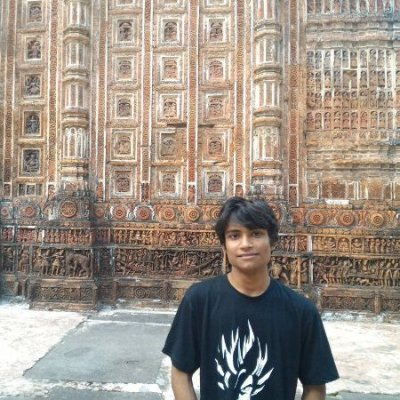
\includegraphics[width=0.15\textwidth]{pp.jpg}
%\end{wrapfigure}

\MyName{Masum Billal}
\MySlogan{Curriculum Vitae}

\sepspace

%%% Personal details
%%% ------------------------------------------------------------
\NewPart{Personal details}{}

\PersonalEntry{Birth}{December 9, 1993}
\PersonalEntry{Address}{47/2, North Mugda, Dhaka-1214}
\PersonalEntry{Phone}{(+88) 01779788023}
\PersonalEntry{Mail}{\url{billalmasum93@gmail.com}}

%%% Education
%%% ------------------------------------------------------------
\NewPart{Education}{}


\EducationEntry{BSc. Engineering}{Final year}{Department of Computer Science and Engineering,\\University of Dhaka}{}

%%% Work experience
\NewPart{Work Experience}
\WorkEntry{Threat Equation PTE LTD.\\Singapore}{April $2016$ - September $2016$}{Remote job as Data Analyst}{}

%%% ------------------------------------------------------------
\NewPart{Publication, Achievements}{}

\EducationEntry{AIST Conference}{2015}{Coauthor of the paper `Similarity Aggregation for Collaborative Filtering' on recommender systems - \texttt{http://link.springer.com/chapter/10.1007/978-3-319-26123-2\_23}}

\EducationEntry{Eureka}{$2014$} {Author of the article `A Nice Theorem in Multiplicative Functions', published on the Journal of Cambridge University, \textit{Eureka}(2014).}

\EducationEntry{Mathematical Reflections}{2012} {Author of the article `Exponent GCD Lemma', published on Mathematical Reflection, issue $6$ ($2012$).}

\EducationEntry{Bangladesh Mathematical Olympiad}{$2010$}{Medal in National and Regional Olympiads}

\EducationEntry{Bangladesh Mathematical Olympiad}{$2009$}{Medal at Regional Olympiad}

\EducationEntry{College Olympiads}{2009-2010}{Several Medals and crests in some olympiads arranged by some local colleges}

\NewPart{Volunteer Experience}
\WorkEntry{Bangladesh Mathematical Olympiad}{$2011$ - $2015$}{Trainer and mentor at Bangladesh National Math Camp and IMO-camp}

\sepspace


\NewPart{Hobbies and Interests}
\SkillsEntry{}{Finding new results on topics I am interested in.}
\SkillsEntry{}{Publications in journals.}
\SkillsEntry{}{Problem setting in mathematics and programming.}
%%% Skills
%%% ------------------------------------------------------------
\NewPart{Skills}{}

\SkillsEntry{Languages}{Bengali (mother tongue)}
\SkillsEntry{}{English}
\vspace{.2in}
\SkillsEntry{Knows}{\textsc{C, C++, Python (Django), PHP, Java, MySQL, Git, \LaTeX}}
\SkillsEntry{}{Front-end languages: \textsc{HTML, CSS, Javascript, Jinja2}, jQuery}
\vspace{.2in}
\SkillsEntry{}{Participated in three ICPC regional contests }
\SkillsEntry{Programming}{and several national programming contests.}
\vspace{.2in}
\SkillsEntry{Data}{\textbf{A Movie Recommender System (Python)}}
\SkillsEntry{Science}{\texttt{https://github.com/fifaboy/rec-mnb}}
\vspace{.1in}
\SkillsEntry{}{\textbf{Online Anime Store (Python, Django)}}
\SkillsEntry{}{\texttt{https://github.com/fifaboy/otaku-store}}
\vspace{.1in}
\SkillsEntry{Projects}{\textbf{Get Github User Information (Python, Django)}}
\SkillsEntry{}{\texttt{https://github.com/fifaboy/git-public-info}}
\vspace{.1in}
\SkillsEntry{}{\textbf{Online Library (Java, JSP)}}
\SkillsEntry{}{\textbf{File Tracker (PHP, Codeigniter)}}
\vspace{.2in}
\SkillsEntry{LinkedIn}{\texttt{https://www.linkedin.com/in/billalmasum93}}
\SkillsEntry{Git Profile}{\texttt{https://github.com/fifaboy}}
\SkillsEntry{Blog}{\texttt{https://karushib.wordpress.com/}}


%%% References
%%% ------------------------------------------------------------
\NewPart{References}
Mahbub Majumdar\\
Professor \\
Computer Science \& Engineering Department\\
BRAC University\\
Buidling-5, Floor-4th, Room: UB50402\\
45 Mohakhali C/A, Dhaka, Bangladesh\\
%Tel: +8804478444060, Ext: 5065\\
Email: \texttt{majumdar@bracu.ac.bd}
\end{document}
